\documentclass[a4paper]{article}
\usepackage[ngerman]{babel} 
\usepackage[utf8x]{inputenc}
\usepackage{tabularx}
\usepackage{booktabs}
\usepackage[table]{xcolor}
\usepackage{xcolor}
\usepackage{graphicx}
\usepackage{hyperref}
\usepackage{amsmath}
\usepackage{float}
\usepackage{listings}
\usepackage{enumitem}
\hypersetup{colorlinks=true,citecolor=black,filecolor=black,linkcolor=black,urlcolor=black}
\usepackage[absolute,overlay]{textpos}
\usepackage{multimedia}
\usepackage{array}
\usepackage[authoryear,square]{natbib}
\usepackage[automark,headsepline]{scrlayer-scrpage}
\pagestyle{scrheadings}
\ihead[]{Powerpoint zu LaTeX Beamer Konverter}
\ohead[]{\today}
\cfoot[]{\pagemark} 	
\setlist[itemize,1]{label=$\cdot$}

\begin{document}
	\pagenumbering{gobble}
	\title{
		\begin{figure}[!ht]
			
\includegraphics[width=0.26\textwidth]{img/TH_Koeln_Logo.pdf}
		\end{figure}
		\vspace{1cm}
		\Huge Powerpoint zu LaTeX Beamer Konverter \\
	}
	
	\vspace{1cm}
	
	\author{\Large \href{mailto:ivan.kurilin@smail.th-koeln.de}{Ivan Kurilin}
		\vspace{1cm}}
		
	
	\date{
		\large Modul: Cyber-Physische Systeme \\
		\vspace{0.8cm}
		\large Prüfer: Prof. Dr. Daniel Gaida \\
		\vspace{1cm}
		\today
	}
	
	\maketitle
	
	\setlength{\parindent}{0pt}
	\newpage
	\begin{abstract}
		Dieser Bericht dokumentiert die Entwicklung eines Tools zur Konvertierung von PowerPoint-Präsentationen in LaTeX-Beamer-Code. Durch die Kombination von \textit{Docling} für die Inhaltsanalyse und lokalen \textit{Large Language Models}  wird eine Pipeline realisiert, die Texte, Medien und Layout-Informationen extrahiert und in kompilierbaren LaTeX-Code überführt. 
	\end{abstract}

	
	
	\newpage
		\tableofcontents
	\newpage
	
	\pagenumbering{arabic}
\section{Einleitung}

In vielen professionellen oder akademischen Umgebungen sind Präsentationen das primäre Medium zur Vermittlung verschiedener Konzepte. Die Software zur Erstellung dieser Präsentationen verfügt über einen hohen Funktionsumfang und eine etablierte Nutzerschaft. Während Microsoft PowerPoint aufgrund der grafischen Benutzeroberfläche und der Geschwindigkeit beim Layouting dominiert, bleibt LaTeX Beamer der bevorzugte Standard für den  Einsatz im MINT Bereich. \\

 Oft werden erste Entwürfe schnell in PowerPoint erstellt. Wenn diese Inhalte später in ein LaTeX Dokument überführt werden müssen, gibt es bisher nur wenige Lösungen. Die manuelle Neuerstellung der Folien ist ein repetitiver und zeitintensiver Prozess. Entwickler müssen Texte kopieren, Tabellenumgebungen händisch programmieren und Bilder positionieren. Diese Arbeit bietet keinen kreativen Mehrwert und hält von den eigentlichen technischen Aufgaben ab. \\

Bisherige Ansätze zur Automatisierung scheitern meist an der Komplexität der Quelldateien. Einfache Parser können die visuelle Anordnung auf einer Folie nicht interpretieren. Sie erkennen zwar den Text, aber nicht die logische Zusammengehörigkeit von Elementen. Eine Liste wird oft nur als loser Textblock extrahiert und die Tabellenstruktur geht vollständig verloren. Ohne ein Verständnis für das Layout muss der generierte Code so stark nachbearbeitet werden, dass der Vorteil der Automatisierung entfällt. Ein detaillierter Vergleich der verschiedenen Tools findet sich in Kapitel 3. \\

Ziel dieses Projekts ist die Entwicklung einer Pipeline, die diesen Prozess durch den Einsatz von künstlicher Intelligenz automatisiert. Durch die Kombination von Layout Analysis und Sprachmodellen soll die visuelle Struktur einer PowerPoint Folie erkannt und direkt in validen LaTeX Code übersetzt werden. Der Fokus liegt dabei auf der korrekten Rekonstruktion von Tabellen, Listen und der absoluten Positionierung von Elementen. Das Tool soll die Geschwindigkeit der grafischen Erstellung mit der typografischen Variabilität von LaTeX vereinen und den manuellen Aufwand auf ein Minimum reduzieren. 
\subsection{Theoretische Grundlagen von pptx Datei} 

Eine .pptx Datei ist weit mehr als nur das visuelle Dokument, das während einer Präsentation auf dem Bildschirm erscheint. Seit der Einführung des Office Open XML Standards durch Microsoft im Jahr 2007 handelt es sich bei diesem Dateiformat technisch gesehen um einen Container \citep{MSOpenXML}. Die Datei ist ein komprimiertes Archiv, das mit einem gewöhnlichen Tool zur Datenkompression entpackt werden kann. Nach dem Entpacken wird die gesamte interne Struktur der Präsentation sichtbar, die aus einer hierarchischen Anordnung von Verzeichnissen und Dateien besteht. \\

Innerhalb dieser Archivstruktur werden die Informationen nicht als ein einziger Datenblock gespeichert, sondern liegen als separate Einheiten vor. Der Kern der Präsentation befindet sich im Verzeichnis für die Folien, in dem jede einzelne Folie als eigene XML Datei gespeichert ist. Diese XML Dateien enthalten die gesamte Logik über die Anordnung von Texten sowie die Definition von grafischen Formen. Die Trennung der Inhalte in einzelne Dateien ermöglicht es einer Pipeline, gezielt auf bestimmte Folien zuzugreifen, ohne das gesamte Dokument verarbeiten zu müssen. \\

Zusätzlich zur Struktur der Folien enthält das Archiv einen speziellen Ordner für Medien. Hier werden sämtliche Assets wie Bilder im Format png oder Videos im Format mp4 als eigenständige Dateien abgelegt. Diese Dateien liegen dort in ihrer ursprünglichen Form vor und sind über Referenzen in den XML Dokumenten mit den jeweiligen Folien verknüpft. Diese modulare Bauweise ist die technische Voraussetzung dafür, dass Bilder und andere Medienformate automatisiert extrahiert und in andere Zielformate wie LaTeX überführt werden können. Die Metadaten über die Dateitypen und die Beziehungen zwischen den Objekten sind in speziellen Beziehungsdateien hinterlegt, die das Mapping innerhalb der Präsentation steuern. 

\subsection{Struktur von OpenXML-Präsentationen} 

Die Architektur von OpenXML basiert auf dem Prinzip der Trennung von Inhalten und deren Beziehungen. Während die eigentlichen Daten in XML Dateien gespeichert werden, steuern separate Beziehungsdateien mit der Endung .rels die Verknüpfungen zwischen den einzelnen Komponenten. Für die Entwicklung einer Pipeline ist diese Abstraktionsebene entscheidend, da ein Objekt auf einer Folie nicht direkt eingebettet ist, sondern über eine eindeutige ID referenziert wird. (s. Abbildung 1 und 2) \\

Innerhalb der Folien XML Dokumente werden grafische Elemente über die Sprache DrawingML \citep{DrawingMLOverview} definiert. Jedes Element wie ein Textfeld oder eine geometrische Form wird als Shape Objekt deklariert \citep{Wordprocessing}. Diese Objekte enthalten Informationen über ihre Geometrie, die Position auf dem Koordinatensystem der Folie sowie die visuellen Eigenschaften. Ein besonderes Merkmal ist die hierarchische Struktur der Textkörper innerhalb dieser Shapes. Texte werden in Absätze und Textläufe unterteilt, was eine präzise Extraktion der Formatierungen ermöglicht. Für den Konverter bedeutet dies, dass die logische Baumstruktur des XML Dokuments traversiert werden muss, um die Inhalte in der richtigen Reihenfolge zu erfassen. \\

Ein weiterer Bestandteil sind die Master Layouts. Diese befinden sich physisch im Verzeichnis ppt/slideMasters und definieren die globalen Platzhalter sowie die Standardformatierungen für eine Gruppe von Folien. Die Pipeline muss in der Lage sein, diese Vererbungslogik zu interpretieren, um statische Elemente von dynamischen Inhalten zu unterscheiden.  \\
\newpage
\begin{figure}[H]
	\centering
	
	\caption{Repräsentation des Bildobjekts in der XML Baumstruktur.\\}
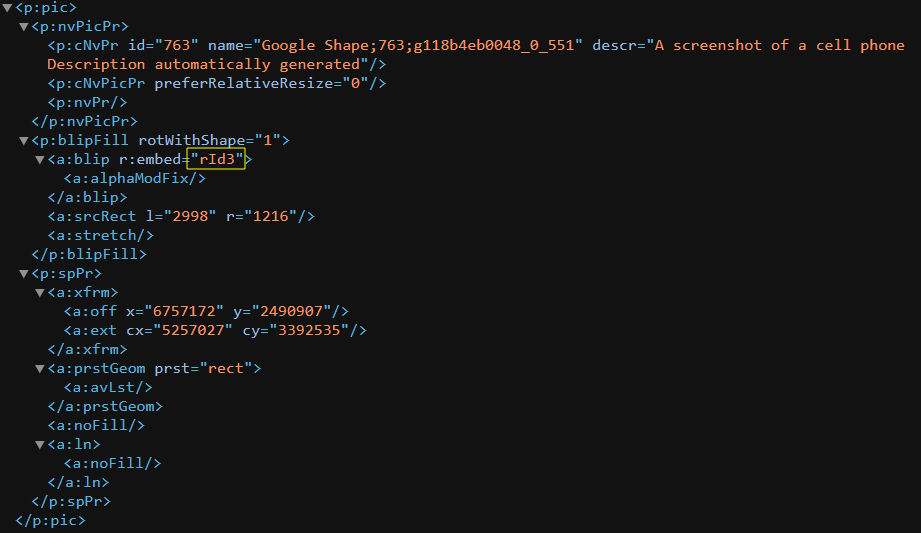
\includegraphics[width=0.9\textwidth]{img/xmlPic.png}
	\label{fig:xml_tree_detail}
	
	\vspace{1cm} 
	
	
	\caption{Referenzierung auf das Bild in der .rels Datei.\\}
	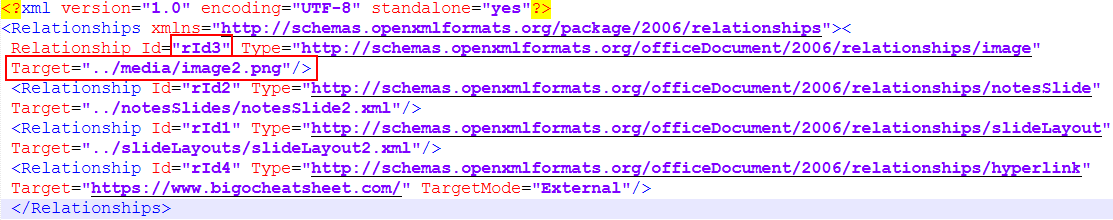
\includegraphics[width=0.9\textwidth]{img/relsPic.png}
	\label{fig:rels_pic_detail}
\end{figure}



\subsection{Herausforderungen der Dokumentenanalyse} \label{sub:doc_analysis}


Die Vorverarbeitung von unstrukturierten Daten für ein Sprachmodell ist die Engstelle der Entwicklungspipeline. Die Datenstruktur ist hierbei die essenzielle Grundlage für die nachfolgende Verarbeitung durch das Large Language Model. Ohne eine geeignete Vorbereitung der Daten und deren strukturierte Nutzung anhand klar definierter Regeln ist es kaum möglich, eine konstante und deterministische Antwort vom Modell zu erhalten. Ein ungeordneter Datenstrom ohne präzise Segmentierung der Layout-Elemente führt dazu, dass das Modell den logischen Kontext verliert, wodurch sich die Qualität der Codegenerierung massiv verschlechtert. 

Auf dem Markt existieren verschiedene Frameworks, die sich auf das Parsing von Dokumenten spezialisiert haben. Ein weit verbreitetes Tool in der Open Source Community ist Unstructured.io \citep{UnstructuredIO}, das besonders häufig für die Entwicklung von RAG-Systemen eingesetzt wird. Daneben bietet IBM Research mit dem Framework Docling \citep{DoclingAI} eine Lösung an, die mittels Deep Learning Modellen spezifisch auf die Erkennung von Tabellen und Koordinaten ausgerichtet ist. 


Die Auswahl des passenden Parsers ist entscheidend für die Stabilität des gesamten Workflows. Jede dieser Bibliotheken verfolgt unterschiedliche Ansätze bei der semantischen Klassifizierung von Objekten. Während einige Frameworks auf starren Heuristiken basieren, nutzen moderne Lösungen neuronale Netze für die Layout-Erkennung. Die Entscheidung für ein Tool beeinflusst maßgeblich, wie präzise die Informationen über die absolute Positionierung der Elemente für die anschließende Generierung erhalten bleiben. Eine detaillierte Gegenüberstellung der Leistungsmerkmale und eine Bewertung für den spezifischen Einsatz in der Konvertierung von Präsentationsmedien findet sich im Kapitel 2 dieser Arbeit. \\



\subsection{Large Language Models in der Codegenerierung}

Nachdem die Dokument-Analyse eine strukturierte Basis geschaffen hat, fungieren Large Language Models als generative Instanz zur Übersetzung dieser Informationen in valide Information. Im Gegensatz zu klassischen, regelbasierten Transpilern, die bei komplexen Verschachtelungen oft an Grenzen stoßen, können moderne Modelle semantische Zusammenhänge interpretieren und in die Ziel-Syntax von LaTeX überführen.


Die zentrale Stärke dieser Modelle liegt in der Fähigkeit zum In-Context Learning. Dabei muss das Modell nicht explizit für die Struktur von PowerPoint-Dateien trainiert werden. Stattdessen werden die extrahierten Metadaten und Koordinaten innerhalb des Prompts so aufbereitet, dass das Modell die räumliche Anordnung der Elemente versteht und in entsprechende LaTeX-Umgebungen übersetzt. Ein kritischer Aspekt in diesem Prozess ist die Syntax-Stabilität. Da die Ausgabe von Sprachmodellen stochastisch erfolgt, ist die Implementierung von Mechanismen zur Validierung des generierten Codes notwendig, um Kompilierungsfehler in der LaTeX-Umgebung zu vermeiden.

In dieser Pipeline übernehmen LLMs somit die Rolle eines intelligenten Compilers, der die Brücke zwischen der rein geometrischen Beschreibung einer Folie und der logischen Strukturierung eines wissenschaftlichen Dokuments schlägt. Die Effizienz dieses Schritts hängt maßgeblich davon ab, wie präzise die Tokenisierung der Eingabedaten erfolgt, um das Kontext-Fenster optimal zu nutzen und Halluzinationen bei der Positionierung von Elementen zu minimieren.

\section{Analyse genutzter Technologien}
\label{sec:tech_analysis}


Die Auswahl einer geeigneten Extraktions-Engine ist die kritischste Design-Entscheidung für die Stabilität und Genauigkeit der Konvertierungspipeline. In diesem Kapitel werden die technologischen Ansätze untersucht, die für die Überführung von unstrukturierten Präsentationsdaten in ein maschinenlesbares Format infrage kommen. Da die Qualität des generierten LaTeX-Codes direkt von der Integrität der Eingangsdaten abhängt, liegt der Fokus des Vergleichs auf der präzisen Erkennung von Layout-Elementen, deren hierarchischen Relationen und der direkten wiedervewendung für das LLM.

Hierbei werden insbesondere die Frameworks Unstructured und Docling gegenübergestellt, die im Bereich der Dokumentenanalyse als führende Open-Source-Lösungen gelten. Durch eine systematische Analyse ihrer Funktionsweisen und Einschränkungen wird die technologische Basis für den anschließenden Systementwurf definiert. Ziel ist es, das Framework zu identifizieren, das die höchste Konsistenz bei der Extraktion von Tabellen, Listen und absoluten Positionen bietet, um den Determinismus des nachgelagerten Sprachmodells zu gewährleisten.


\subsection{Evaluation der Extraktionsverfahren}
\label{sub_swot_analysis}

\begin{table}[h]
	\centering
	\caption{SWOT-Analyse der Extraktions-Technologien}
	\label{tab:swot_comparison}
	\begin{tabularx}{\textwidth}{l X X}
		\toprule
		\rowcolor{gray!10} Kategorie & Docling & Unstructured.io \\
		\midrule
		Stärken & Erkennung von Tabellenstrukturen und geometrischen Anordnungen. & Hohe Bekanntheit und breite Unterstützung verschiedener Dateiformate in der Community. \\
		\addlinespace
		Schwächen & Fehlende Unterstützung für die Extraktion von eingebetteten Mediendateien wie .mp4-Videos. & Kostenfreie Nutzung eingeschränkt; erfordert Account und API-Key. Keine Bereitstellung von Bounding-Box-Koordinaten zur Weiterverarbeitung. \\
		\addlinespace
		Chancen & Nahtlose Integration in lokale Pipelines; ermöglicht volle Kontrolle über den Datenfluss ohne externe Cloud-Abhängigkeit. & Schnelle Skalierbarkeit in Cloud-Umgebungen durch fertige API-Schnittstellen. \\
		\addlinespace
		Risiken & Projektfortschritt hängt von der Wartung der spezifischen IBM-Modelle ab. & Langfristige Abhängigkeit von Preismodellen und Lizenzänderungen des Anbieters. \\
		\bottomrule
	\end{tabularx}
\end{table}

Wie die Analyse zeigt, bietet keines der betrachteten Tools eine vollständig deckungsgerechte Lösung für die Konvertierung von PowerPoint zu LaTeX. Ein massives Problem in der praktischen Anwendung ist die enorme Datenmenge: Bereits ein mittelkomplexes Dokument resultiert nach dem Parsing oft in mehreren tausend Zeilen JSON-Code pro Folie. Dieser Overhead überfüllt das Context Window des Sprachmodells, wodurch die Präzision der Antwort sinkt und das Risiko für Halluzinationen steigt.

Um eine konstante und deterministische Ausgabe zu garantieren, ist eine radikale Minimierung der Datenmenge unumgänglich. Es ist notwendig, ein proprietäres JSON-Objekt zu konstruieren, das ausschließlich die für die LaTeX-Generierung kritischen Attribute (wie Textinhalt, relative Position und Tabellenstruktur) filtert. In diesem Zusammenhang muss kritisch geprüft werden, ob eine direkte Extraktion über die Bibliothek python-pptx \citep{PythonPptxDoc} langfristig effizienter ist. Dieser Ansatz würde es erlauben, die JSON-Struktur von Grund auf selbst zu definieren und so den Abhängigkeitsfaktor zu externen Frameworks zu minimieren.

Eine detaillierte Darstellung der entwickelten JSON-Strukturen sowie die Validierung der daraus resultierenden Konvertierungsqualität erfolgt im Kapitel 4 bei den Ergebnissen.

\subsection{Inferenz-Infrastruktur}

Die lokale Bereitstellung des LLMs erfordert eine Inferenz-Infrastruktur, welche die Modellverwaltung sowie die Kommunikation mit der Pipeline übernimmt. Im Rahmen dieses Projekts wurde {Ollama} als primäres Framework gewählt. 

Die Entscheidung für Ollama basiert auf mehreren funktionalen Vorteilen:

Das Framework ermöglicht den Zugriff auf eine Vielzahl vorkonfigurierter Modelle sowie eine einfache Installation und Aktualisierung.

Durch die Bereitstellung einer lokalen REST-Schnittstelle lässt sich Ollama nahtlos in die bestehende Python-Applikation integrieren.

 Die zugehörige Applikation erlaubt es, Prompts vorab interaktiv zu evaluieren. Da die Inferenz-Parameter in dieser Testumgebung identisch mit der API-Schnittstelle sind, ist eine hohe Konsistenz der Ergebnisse zwischen Testphase und produktiver Anwendung gewährleistet.\\


Als weitere technologische Möglichkeit auf dem Markt existiert zudem {LM Studio} \citep{LMStudio}. Ein wesentlicher Unterschied liegt hier in der Kontrolle über die Hardware-Ressourcen. Im Gegensatz zu Ollama erlaubt LM Studio die explizite Zuweisung von Systemspeicher oder Grafikspeicher für das jeweilige Modell, was insbesondere bei spezifischen Hardware-Optimierungen von Vorteil sein kann. Für den Workflow dieser Arbeit deckte Ollama jedoch alle notwendigen Anforderungen an die Automatisierung und Stabilität vollständig ab.

\subsubsection{Modellwahl}

Die Auswahl des Sprachmodells ist maßgeblich für die Qualität des generierten {LaTeX}-Codes verantwortlich. Da die Inferenz lokal durchgeführt wird, ist die Modellwahl jedoch direkt an die Hardware-Ressourcen des Test-Systems gebunden. Aufgrund der verfügbaren Rechenleistung stieß das System bei Modellen mit einer Parametergröße von ca. 8 Milliarden (8B) an seine Leistungsgrenzen, weshalb der Fokus auf Modellen in dieser Größenordnung lag.

Im Rahmen der Evaluation wurden verschiedene Modelle getestet:
\begin{itemize}
	\item {deepseek-r1:8b:} Trotz der hohen Bekanntheit von DeepSeek im Web konnten diese Modelle für die Code-Generierung in diesem spezifischen Kontext keine ausreichend konsistenten Ergebnisse liefern \citep{deepseek}.
	\item {qwen3:8b:} Dieses Modell lieferte qualitativ hochwertige Ergebnisse. Da es sich hierbei jedoch um ein \texttt{Thinking} -Modell handelt, lag die Verarbeitungszeit bei ca. zwei bis drei Minuten pro Folie. Diese Inferenzgeschwindigkeit erwies sich für den Betrieb einer zeiteffizienten automatisierten Pipeline als unzureichend \citep{Qwen3}.
	\item {qwen2.5-coder:7b:} Dieses Modell stellte sich als optimaler Kompromiss heraus. Es lieferte eine zum 8B-Modell gleichwertige Code-Qualität, reduzierte die Verarbeitungszeit jedoch signifikant auf ca. 20 bis 30 Sekunden pro Folie \citep{Qwen25Coder}. 
\end{itemize}

Der direkte visuelle Vergleich (siehe Abbildungen \ref{fig:qwen3_8b} und \ref{fig:qwen2_5_coder_7b}) verdeutlicht, dass das spezialisierte Coder-Modell trotz geringerer Parameteranzahl präzisere Strukturen erzeugt.

\begin{figure}[H]
	\centering
	
	\caption{Generierungsergebnis des Qwen3-Modells (8B)}
	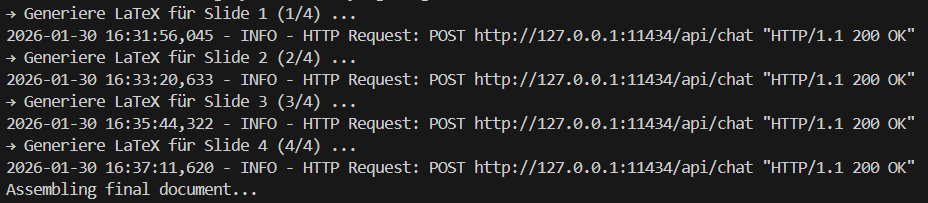
\includegraphics[width=0.9\textwidth]{img/qwen3_8b.png}
	\label{fig:qwen3_8b}
	
	\vspace{2em} 
	
	\caption{Generierungsergebnis des Qwen2.5-Coder-Modells (7B)}
	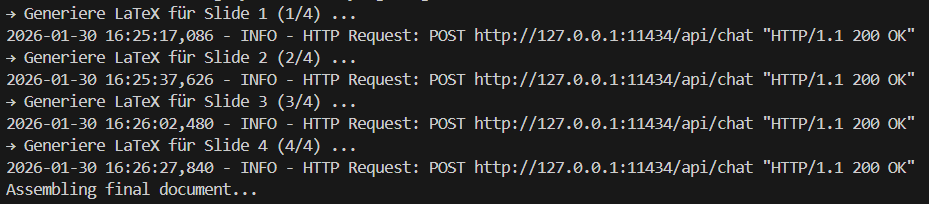
\includegraphics[width=0.9\textwidth]{img/qwen2_5_coder_7b.png}
	\label{fig:qwen2_5_coder_7b}
\end{figure}

\subsection{Unabhängigkeit von Cloud-Modellen}

Der Einsatz von Large Language Models erfolgt in der Praxis häufig über Cloud-Schnittstellen großer Technologieunternehmen wie OpenAI, Google oder Microsoft. Diese Abhängigkeit von externen Infrastrukturen bringt jedoch signifikante Risiken im Hinblick auf die Datensicherheit mit sich. In dieser Arbeit wird daher ein konsequent dezentraler Ansatz verfolgt, der durch die Nutzung von Ollama die Inferenz vollständig auf lokaler Hardware realisiert.

Ein wesentlicher Aspekt ist der Schutz geistigen Eigentums. Insbesondere im akademischen Kontext enthalten Präsentationen oft unveröffentlichte Forschungsergebnisse oder sensible Konzepte. Die Übermittlung dieser Daten an externe Server ist aus Datenschutzsicht kritisch zu bewerten. Durch die lokale Ausführung wird garantiert, dass keine Inhalts-Fragmente die eigene Infrastruktur verlassen. Darüber hinaus sichert dieser Ansatz die Unabhängigkeit von den Preismodellen und der Verfügbarkeit kommerzieller Anbieter. 

\section{Systementwurf und Architektur}

Dieses Kapitel behandelt die softwaretechnische Architektur des Konverters und die zugrunde liegenden Entwurfsentscheidungen. Das primäre Ziel des Systems ist die automatisierte Transformation von Präsentationsdaten in satzfähige LaTeX-Beamer-Dokumente. Der Entwurf basiert auf einer modularen Pipeline-Struktur, die eine strikte Trennung zwischen Datenextraktion, Prozessierung und Codegenerierung sicherstellt.


\subsection{Pipeline-Konzept und Modulbauweise} 
Die Implementierung der Systemarchitektur erfolgt nach dem Pipe-and-Filter-Entwurfsmuster. Diese Wahl ermöglicht die Dekomposition des Transformationsprozesses in diskrete, austauschbare Funktionseinheiten. Der Datenfluss beginnt mit der Auflösung der OpenXML-Struktur der Quelldatei. Hierbei agieren die Medienextraktion und die Layout-Analyse als initiale Filter, welche die Rohdaten in ein internes Repräsentationsformat überführen.

Durch diese modulare Entkopplung wird die Robustheit des Gesamtsystems gegenüber heterogenen Eingangsdaten erhöht. Ein wesentlicher Vorteil dieser Architektur liegt in der Unabhängigkeit der Prompt-Konstruktion von der physischen Datenextraktion. Die Kommunikation zwischen den einzelnen Filtern erfolgt über standardisierte Schnittstellen, was die Konsistenz der Datenströme über die gesamte Prozesskette hinweg gewährleistet und die Grundlage für eine deterministische Generierung des Zielcodes bildet.
\subsection{Extraktions-Layer}

Der Extraktions-Layer fungiert als Schnittstelle zwischen dem OpenXML-Containerformat und der internen Datenverarbeitung der Pipeline. Die primäre Aufgabe besteht in der Aggregation semantischer Informationen und der Isolation eingebetteter Ressourcen. Um eine vollständige Erfassung aller Folienobjekte bei gleichzeitiger Optimierung des Datenvolumens sicherzustellen, implementiert das System eine hybride Extraktionsstrategie. Diese unterteilt sich in die Analyse der logischen Dokumentenstruktur und die physische Sicherung der Mediendaten.

\subsubsection{Strukturanalyse}

Die strukturelle Analyse der Präsentationsdatei wird primär durch das Framework Docling realisiert. Dieses Modul übernimmt die Transformation der Folienhierarchie in ein JSON-Format, wobei Textelemente, Listenstrukturen und Tabellen klassifiziert werden.

Ein technisches Hindernis bei der Verwendung von Docling besteht in der Serialisierung grafischer Elemente als Base64-kodierte Zeichenfolgen. Da dies zu einer signifikanten Vergrößerung des Datenstroms führt und die Performance bei der späteren Interaktion mit Sprachmodellen reduziert, findet eine gezielte Bereinigung statt. Die strukturellen Informationen werden von den Bilddaten entkoppelt. Ergänzend dazu wird die Bibliothek python-pptx eingesetzt, um einen Zugriff auf die zugrunde liegenden XML-Knoten der Office Open XML-Spezifikation zu erhalten. Diese Kombination ermöglicht es, die durch Docling erzeugte Struktur mit Metadaten und Pfadreferenzen anzureichern, während das Rauschen innerhalb des Datenmodells minimiert wird.

\subsubsection{Medien-Extraktion}

Die Implementierung einer eigenständigen Medien-Extraktion ist eine direkte Reaktion auf die funktionalen Limitationen des eingesetzten Frameworks. Da Docling visuelle Inhalte ausschließlich als Base64-kodierte Zeichenfolgen serialisiert und aktuell keine Unterstützung für Video-Objekte bietet, ist eine manuelle Entkopplung dieser Typen erforderlich. Nur so kann die Datenökonomie innerhalb des JSON-Objekts gewahrt werden.

Darüber hinaus erfordert die hierarchische Organisation des OpenXML-Formats eine spezifische Herangehensweise. Da Medienelemente innerhalb der Folienstruktur oft in tief verschachtelten Gruppen organisiert sind, führt eine lineare Verarbeitung zwangsläufig zu einem unvollständigen Datenmodell. Ein rekursiver Algorithmus ist daher die methodische Konsequenz, um die Integrität der extrahierten Ressourcen über alle Ebenen hinweg zu gewährleisten. Durch die anschließende Transformation der absoluten Positionsdaten in ein relatives Koordinatensystem wird die Abhängigkeit von proprietären Maßeinheiten aufgelöst. Diese Normalisierung bildet die Grundlage für eine präzise Rekonstruktion der Layouts innerhalb der LaTeX-Beamer-Umgebung.
\subsection{Datenminimierung}

Die Transformation der Rohdaten in eine Intermediate Representation überführt unterschiedliche Datenstrukturen in ein einheitliches Schema. Durch das Mapping von semantischen Inhalten auf physische Medienreferenzen wird die Komplexität der Quelldaten für die nachfolgende Pipeline reduziert. Diese Konsolidierung verringert die Anzahl der Datenpunkte pro Folie signifikant, was die Performance bei der Verarbeitung durch LLMs steigert. Eine minimierte Datenobjekt stellt sicher, dass das Context Window optimal genutzt wird und die Qualität der Codegenerierung durch ein besseres Signal-Rausch-Verhältnis steigt.
\subsubsection{Koordinatentransformation}
Um die Layout-Integrität beim Export von OpenXML nach LaTeX zu wahren, ist eine Normalisierung der Koordinatensysteme notwendig. PowerPoint nutzt intern English Metric Units, die für eine direkte Verwendung in LaTeX Beamer zu hochauflösend und einheitsabhängig sind. Die Transformation überführt die absoluten Bounding-Box-Werte in ein relatives Koordinatensystem im Intervall $[0.0, 1.0]$.

Dabei werden die Parameter für Position ($x, y$) und Ausdehnung ($w, h$) durch Division mit der gesamten Folienbreite bzw. Folienhöhe berechnet. Diese unit-agnostische Darstellung entkoppelt die Geometrie von festen Maßeinheiten wie pt oder cm und ermöglicht eine konsistente Skalierung innerhalb der Zielumgebung. Die Berechnung stellt zudem sicher, dass vertauschte Extremwerte innerhalb der Metadaten korrigiert werden (siehe Abbildung \ref{fig:code_geometry}).
\begin{figure}[H]
	\centering
	\caption{Python-Implementierung der Normalisierungslogik: Umrechnung absoluter EMUs in relative Koordinaten.\\}
	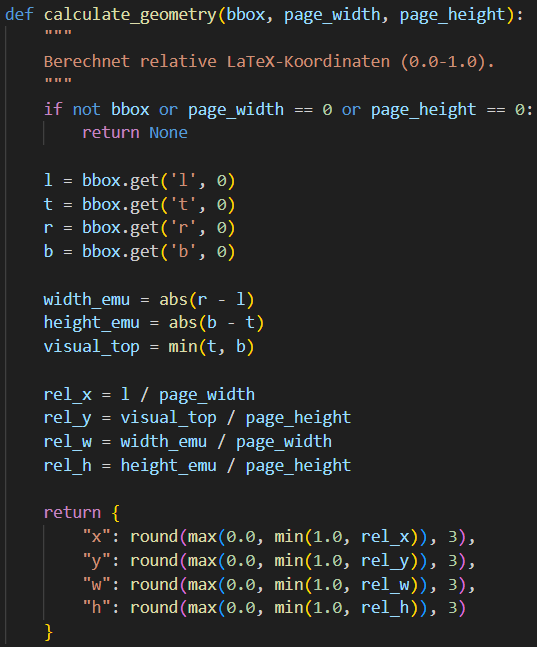
\includegraphics[width=0.6\textwidth]{img/calculate_geometry.png}
	\label{fig:code_geometry}
\end{figure}

\subsubsection{Semantische Anreicherung}

Nach der geometrischen Aufbereitung folgt die Überführung der flachen Elementliste in ein strukturiertes Modell. Da das Ausgangsformat lediglich isolierte Objekte liefert, nutzt die Logik räumliche Heuristiken zur Erkennung von logischen Zusammenhängen. Elemente werden basierend auf ihrer vertikalen Position und ihrer Ausrichtung gruppiert, um Header von Inhaltsbereichen zu differenzieren. Dieser Schritt ist essenziell, um die semantische Hierarchie der Folie wiederherzustellen und Fragmente in kohärente Elementgruppen zu überführen.

Abbildungen \ref{fig:json_raw_transformation}  und \ref{fig:json_cleaned_transformation}   visualisieren diese Transformation am Beispiel eines Titel-Elements. Während der Rohdatensatz tief verschachtelte Metadaten enthält, reduziert die Intermediate Representation diese Komplexität signifikant. Die Klassifikation des Elements als Header erfolgt hier deterministisch durch die Auswertung der normalisierten y-Koordinate ($y < 0.03$). Die Bedingung besagt, dass die Oberkante des Elements in den obersten 3, der gesamten Folienhöhe liegt. 



\begin{figure}[H]
		\centering
	\caption{Vor der Transformation. \\}
	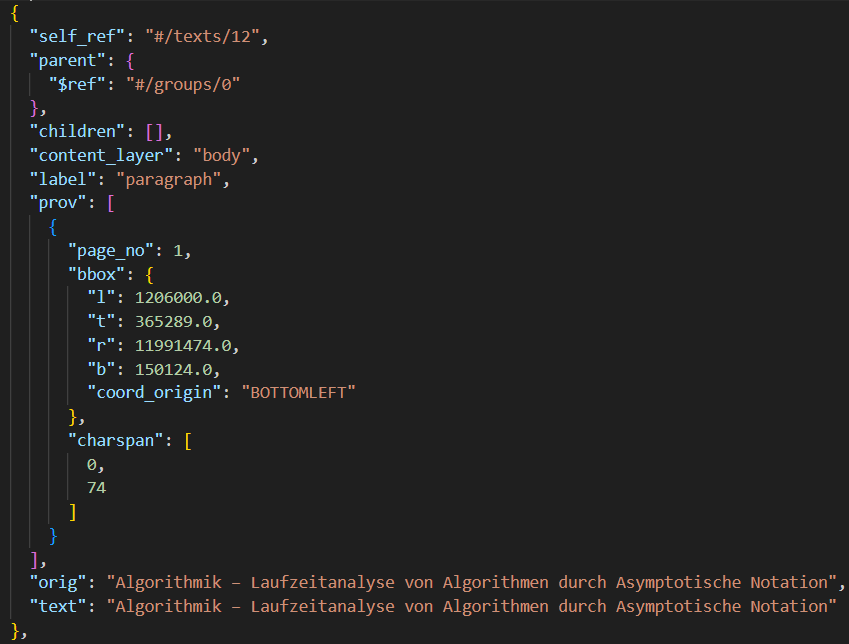
\includegraphics[width=0.9\textwidth]{img/JSON_RAW.png}
	\label{fig:json_raw_transformation}
	
	\caption{Nach der Transformation.\\}
	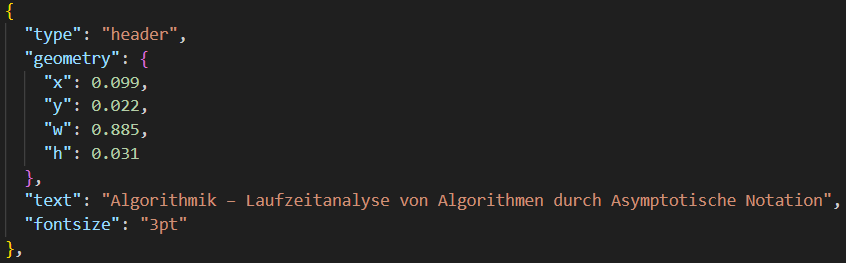
\includegraphics[width=0.9\textwidth]{img/JSON_CLEANED.png}
	\label{fig:json_cleaned_transformation}
		

	
\end{figure}


Diese Strategie instruiert das nachgelagerte Modell, eine korrespondierende Schriftgrößen-Skalierung vorzunehmen, ohne dass explizite Stil-Attribute aus der Quelldatei übernommen werden müssen.

\subsection{Agenten-basierte Synthese}
Die Transformation des Datensatzes in LaTeX-Code ist der vorletzter Schritt der Pipeline. Um die Komplexität zu reduzieren, wird ein modularer Ansatz gewählt, der die Erstellung von Präambel, Folieninhalten und Postambel entkoppelt. Da statische Komponenten wie Paket-Importe oder die Titelfolie effizient als feste Präambel bzw. Postambel definiert werden können, wird die generative Last des Modells gezielt auf die Synthese des eigentlichen Folieninhalts beschränkt.

Die folgenden Unterabschnitte analysieren die Architektur des verwendeten Prompts, der sich aus drei Kernkomponenten zusammensetzt: dem syntaktischen Regelwerk, den exemplarischen Anweisungen und den injizierten Nutzdaten aus dem JSON-Objekt.

\subsubsection{Prompt-Engineering und Methodik}
Die Code-Synthese basiert auf einer  Konditionierung des Sprachmodells, um die Fehleranfälligkeit bei der Generierung LaTeX-Strukturen zu reduzieren. Ein wesentliches Merkmal dieses Prozesses ist die Beschränkung des Kontextfensters auf einzelne Folieneinheiten. Durch diese Verarbeitung wird sichergestellt, dass das Modell während der Inferenz nicht durch globale Dokumentstrukturen abgelenkt wird, was das Risiko für Halluzinationen minimiert.

Der System-Prompt fungiert dabei als syntaktischer Guardrail. Wie in Listing \ref{lst:prompt_rules} dargestellt, wird das Modell durch explizite Instruktionen auf ein vordefiniertes Zielschema fixiert. Ein zentraler Aspekt ist hierbei die Abbildung der normalisierten Geometriedaten ($x, y \in [0,1]$) auf das {textpos}-Paket. Anstatt dem Modell gestalterische Freiheiten zu lassen, erzwingt der Prompt die Kapselung sämtlicher Inhalte in {minipage}-Umgebungen innerhalb definierter {textblock}-Container.

\begin{lstlisting}[basicstyle=\small\ttfamily, frame=lines, caption={Definition des Eingabedatensatzes}, label={lst:prompt_rules}]
{
INPUT DATA:
You receive a JSON object representing a SINGLE slide with a list of "elements".
Each element contains:
"type": text, list, codeblock, table, picture, video, ..
"geometry": { "x", "y", "w", "h" } (Normalized coordinates 0.0-1.0)
"content": "text", "items", "table_rows", "image_path", "path", ..

OUTPUT FORMAT RULES (STRICTLY FOLLOW):
1. **Frame Structure:**
..
2. **Positioning (The Container):**
..
3. **Content Layout (The Inner Box):**
..
4. **Element-Specific Rendering:**
}
\end{lstlisting}

\paragraph{Exemplarische Anweisung:}
Um die Präzision der semantischen Abbildung weiter zu erhöhen, kommen gezielte Input-Output-Beispiele zum Einsatz. Diese decken technische Grenzfälle ab, die über rein deklarative Regeln schwer zu erfassen sind. Beispielsweise lernt das Modell durch diese Paare die typografische Skalierung von Attributen in spezifische Befehle oder die Einbettung von Tabellenstrukturen in {resizebox}-Umgebungen zur Wahrung der strukturellen Integrität. Auch die differenzierte Setzung der Ausrichtungsparameter ({[t]} vs. {[b]}) basierend auf dem semantischen Typ wird durch dieses demonstrative Vorgehen präzisiert (siehe Listing \ref{lst:few_shot_example}).


\begin{lstlisting}[basicstyle=\small\ttfamily, frame=lines, caption={Beispielhafte Instanz für die In-Context-Konditionierung}, label={lst:few_shot_example}]
	Input 2 (List - [b]):
	{
		"type": "list",
		"geometry": {"x": 0.1, "y": 0.2, "w": 0.8, "h": 0.6},
		"items": ["Point A", "Point B"],
		"align": "b"
	}
	
	Output 2:
	\begin{textblock}{0.8}(0.1, 0.2)
		\begin{minipage}[b][0.6\paperheight]{\linewidth}
			\begin{itemize}
				\item Point A
				\item Point B
			\end{itemize}
		\end{minipage}
	\end{textblock}
\end{lstlisting}

Durch das {In-Context Pattern} gewinnt das Modell die in den Beispielen demonstrierte Struktur. Dies verschiebt den Prozess von einer rein generativen Aufgabe hin zu einer geführten Transformation, was die deterministische Stabilität des Outputs deutlich steigert.

\subsection{Syntax-Validierung}


Künstliche Intelligenz generiert Ergebnisse auf Basis von Wahrscheinlichkeiten. Dieses Verhalten führt systembedingt zu Halluzinationen, was auch bei der Erzeugung von LaTeX-Code auftritt. In diesem Abschnitt werden bekannte Fehler abgefangen. Es erfolgt eine gezielte automatisierte Nachbereitung, um typische Flüchtigkeitsfehler in der Syntax zu korrigieren. Mittels regulärer Ausdrücke werden unvollständige Schlüsselwörter wie \textbackslash paper erkannt und zu \textbackslash paperheight ergänzt, um Kompilierungsfehler bei der Positionsbestimmung zu verhindern.\\

Die Implementierung der Steuerzeichen-Bereinigung folgt dem Ziel, die Kompilierstabilität durch deterministische Ersetzungsregeln zu sichern. Da Sprachmodelle aufgrund ihrer Tokenisierung dazu neigen, Backslashes fälschlicherweise als Schrägstriche oder Backspace-Zeichen auszugeben, transformiert die Routine diese Artefakte systematisch in valide LaTeX-Befehle (begin, end, item).

\subsection{Kompilierung} 
Nach der sequenziellen Generierung sämtlicher Folienfragmente erfolgt die finale Aggregation des Dokuments. Hierbei wird der generierte Inhalt mit der initial erzeugten Präambel sowie der Postambel konkateniert, um ein valides {.tex}-Dokument zu bilden. Vor der Persistierung auf dem Dateisystem durchläuft der Quelltext einen Bereinigungsschritt, um potenzielle Inferenz-Artefakte des Sprachmodells zu entfernen.

Der Kompilierungsprozess wird über die {subprocess}-Schnittstelle gesteuert. Die Ausführung der {pdflatex}-Engine erfolgt innerhalb des Zielverzeichnisses, wodurch die korrekte Auflösung relativer Pfade für eingebundene Medienressourcen sichergestellt wird. Zur Gewährleistung einer unterbrechungsfreien Pipeline wird der Compiler im Modus {-interaction=nonstopmode} betrieben. Diese Konfiguration steigert die Robustheit der automatisierten Verarbeitung, da der Satzvorgang bei geringfügigen Fehlern fortgesetzt wird und der Prozess lediglich bei kritischen Syntaxfehlern terminiert [\cite{Eijkhout1991}].
\begin{itemize}
	\item {Validierung}: Die erfolgreiche Erzeugung des PDF-Dokuments dient als primärer Indikator für die syntaktische Korrektheit des generierten Codes.
	\item {Fehlerdiagnose}: Im Falle eines Fehlschlags (Return-Code $\neq$ 0) extrahiert das System die finalen Zeilen der Ursache. Dies ermöglicht eine gezielte Fehleranalyse.
\end{itemize}



\section{Ergebnisse} Das vorliegende Kapitel evaluiert die Leistungsfähigkeit des entwickelten Systems. Im Fokus stehen dabei die Analyse der generierten Artefakte, die Identifikation technischer Limitationen sowie ein abschließender Vergleich mit existierenden Web-Tools.

\subsection{Artefakte und Limitationen} Während der Transformation von PowerPoint-Folien in LaTeX-Code traten spezifische Problemstellungen auf, die die visuelle Treue des Ziel-Dokuments beeinflussen. Diese lassen sich in drei Kategorien unterteilen:

\paragraph{Designelemente:} Ein Problem stellt die Extraktion von freien Formen und spezifischen PowerPoint-Shapes dar. Da diese innerhalb der Datenstruktur oft nur als generische Shapes ohne präzise Pfad-Spezifikationen referenziert werden, ist eine exakte Rekonstruktion in LaTeX aktuell nicht ohne Informationsverlust möglich. Ähnliches gilt für folienübergreifende Design-Templates und Hintergrundfarben: Da diese weder als Bilddateien noch als semantische Objekte extrahiert werden können, beschränkt sich der Output primär auf den funktionalen Content.


\paragraph{Datenintegrität bei der Medienextraktion:} Die Evaluation der Bildextraktion via Docling ergab, dass nicht alle grafischen Inhalte konsistent erkannt werden. Bestimmte Medientypen werden im Extraktionsprozess ignoriert, was zu einem teilweisen Content-Verlust im generierten LaTeX-Dokument führt. Für eine vollständige Dokumentation der Folieninhalte ist hier eine Nachbesserung der Parsing-Logik oder eine alternative Extraktionsmethode notwendig.

\subsubsection{Geometrische Inkonsistenzen bei Verschachtelungen}


Ein technisches Problem bei der Verarbeitung Folienlayouts ist der Umgang mit Gruppierungen. Während einzeln stehende Elemente absolute Koordinaten relativ zum Folienrand besitzen, verhalten sich verschachtelte Elemente in der Datenstruktur anders. Die Extraktion via {python-pptx} erkennt zwar die Gruppierung, liefert für die darin enthaltenen Elemente jedoch Positionsdaten, die sich nicht auf die gesamte Folie beziehen.


Um dieses Verhalten zu untersuchen, wurde eine Folie mit verschachtelten Inhalten (s. Abbildung 8) analysiert. Dabei wurden die Rohdaten desselben Objekts in zwei Zuständen verglichen: einmal als Teil einer Gruppe und einmal nach dem manuellen Auflösen der Gruppierung.

\begin{figure}[H]
	\centering
	
	\caption{Darstellung Slide 7 innerhalb des Powerpoints (Gruppiert)}
	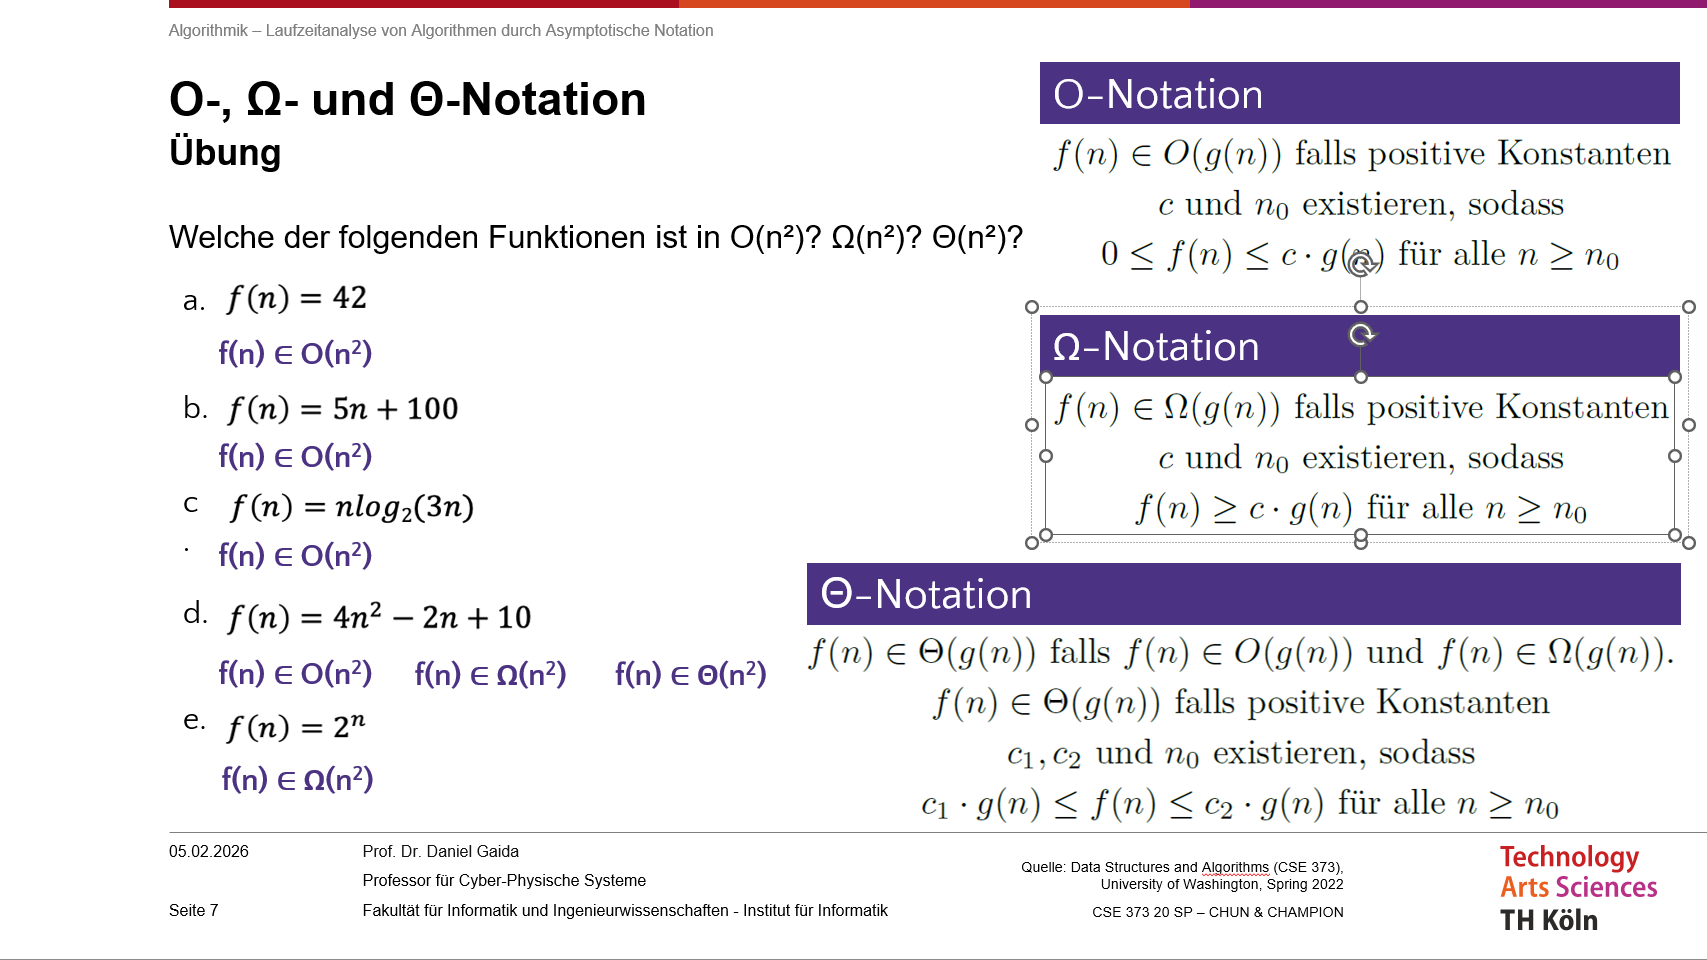
\includegraphics[width=0.9\textwidth]{img/Slide_7_Raw.png}
	\label{fig:Slide 7}
	
\end{figure}

Der Vergleich der Extraktions-Logs in Listing \ref{lst:group_coords} und Listing \ref{lst:ungroup_coords} offenbart die Ursache für die fehlerhafte Darstellung.
In der gruppierten Struktur (Listing \ref{lst:group_coords}) wird das Bildelement {Grafik 36} mit einem {Left}-Wert von ca. $3{,}35\,\mathrm{cm}$ ausgewiesen.

\begin{lstlisting}[caption={Auszug der Rohdaten: Gruppiertes Objekt }, label={lst:group_coords}, basicstyle=\ttfamily\scriptsize]
	Shape: 'Gruppieren 34' (Type: GROUP (6))
		Geo: Left: 7426683 (20.63cm), Top: 453359 (1.26cm) ...
		[!] GROUP DETECTED - Checking Children:
			Shape: 'Grafik 36' (Type: PICTURE (13))
			Geo: Left: 1206500 (3.35cm), Top: 3618076 (10.05cm) ...
\end{lstlisting}

Im Gegensatz dazu zeigt Listing \ref{lst:ungroup_coords} dasselbe Bild (\texttt{Grafik 1}) nach der Auflösung der Gruppe. Hier wird die tatsächliche Position auf der Folie mit ca. $20{,}63\,\mathrm{cm}$ korrekt angegeben.

\begin{lstlisting}[caption={Auszug der Rohdaten: Entkoppeltes Objekt }, label={lst:ungroup_coords}, basicstyle=\ttfamily\scriptsize]
	Shape: 'Grafik 1' (Type: PICTURE (13))
		Geo: Left: 7427146 (20.63cm), Top: 895227 (2.49cm) ...
\end{lstlisting}

Die Daten belegen, dass die Extraktions-Engine bei verschachtelten Objekten lediglich den lokalen Abstand zum inneren Rand der Gruppe misst, nicht jedoch die absolute Position auf der Folie.

Das Problem entsteht bei der Interpretation dieser Werte:
\begin{itemize}
	\item Das Bild befindet sich visuell am rechten Rand der Folie (bei ca. $20{,}63\,\mathrm{cm}$).
	\item Der Parser liefert jedoch den lokalen Wert von ca. $3{,}35\,\mathrm{cm}$, da er den Startpunkt der Elterngruppe ignoriert.
	\item Da unser Algorithmus diesen Wert direkt als globale Koordinate interpretiert, wird das Bild im finalen LaTeX-Dokument fälschlicherweise fast $17\,\mathrm{cm}$ zu weit links platziert.
\end{itemize}

Es handelt sich somit um ein Problem der Referenzierung. Die inneren Elemente einer Gruppe erben nicht den absoluten Startpunkt innerhalb ihres Eltern-Elements, sondern beginnen ihre Zählung in einem eigenen, lokalen Koordinatensystem. Die Übernahme der relativen Koordinaten durch Docling führt zu der in Abbildung \ref{fig:Slide_7_grp_Latex} dargestellten Verschiebung:


\begin{figure}[H]
	\centering
	
	\caption{Layout-Kollaps durch Interpretation relativer Gruppen-Koordinaten als globale Werte.\\}
	\label{fig:Slide_7_grp_Latex}

	\fbox{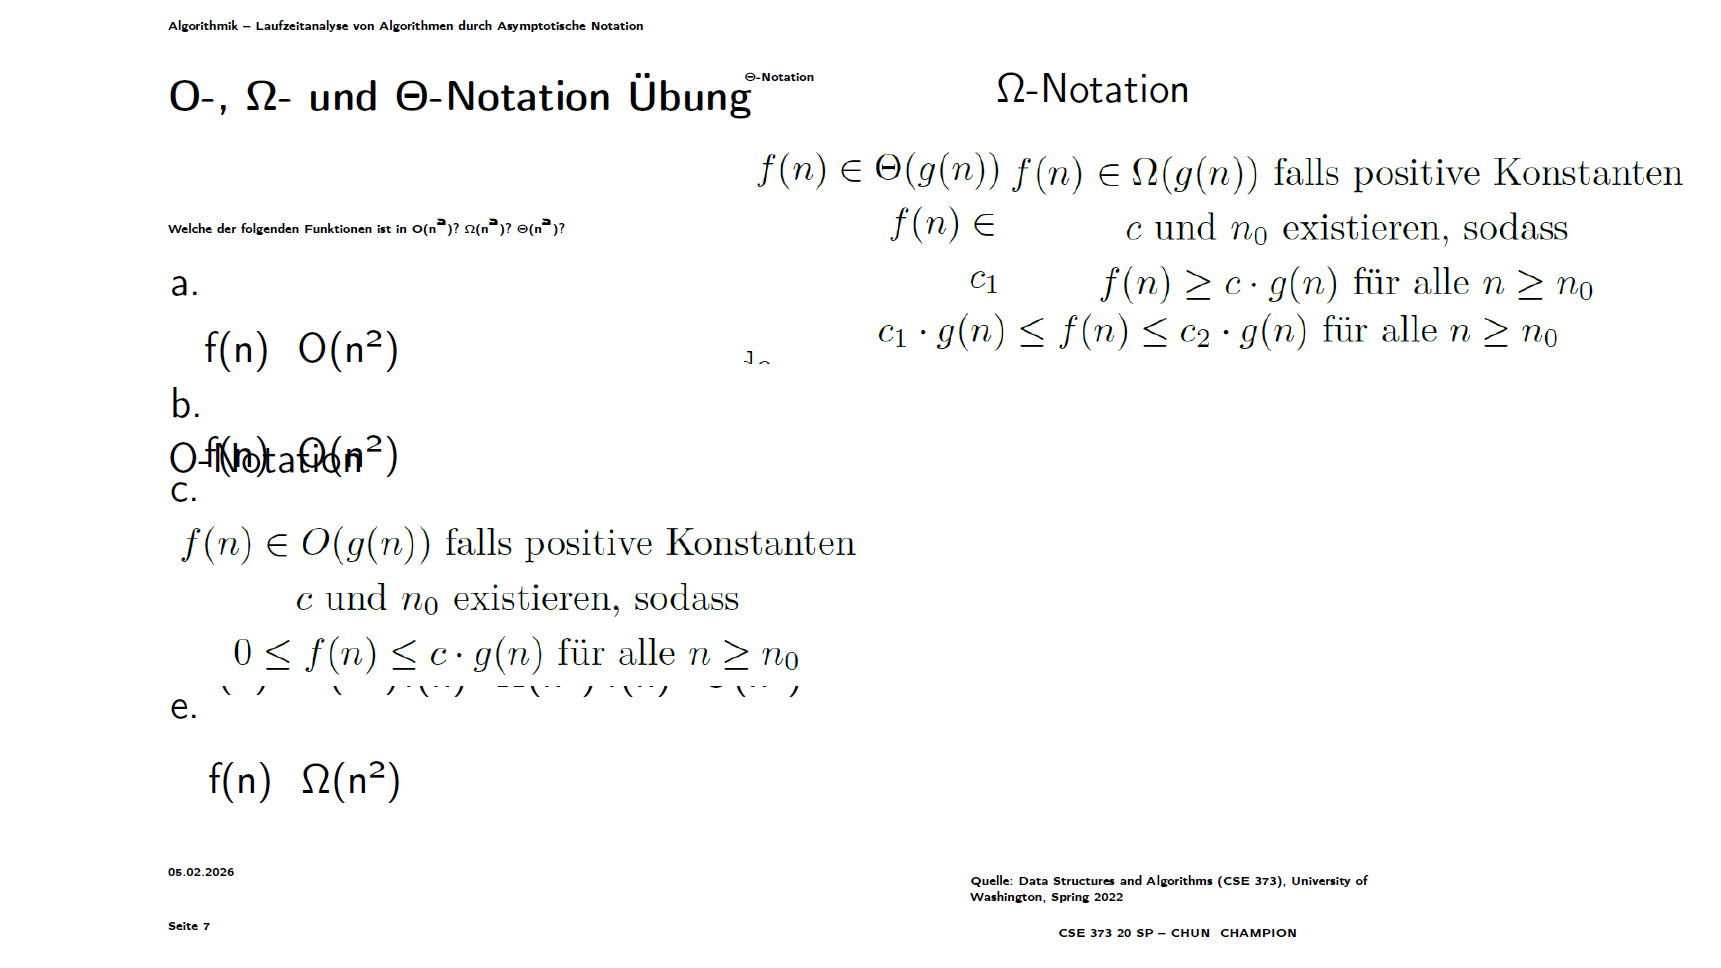
\includegraphics[width=0.95\textwidth]{img/Slide_7_grp_Latex.png}}
	
	\vspace{1cm} 
	

	\caption{Valides Layout nach Auflösung der Gruppierung und Nutzung absoluter Koordinaten.\\}
	\label{fig:Slide_7_non_grp_Latex}
	\fbox{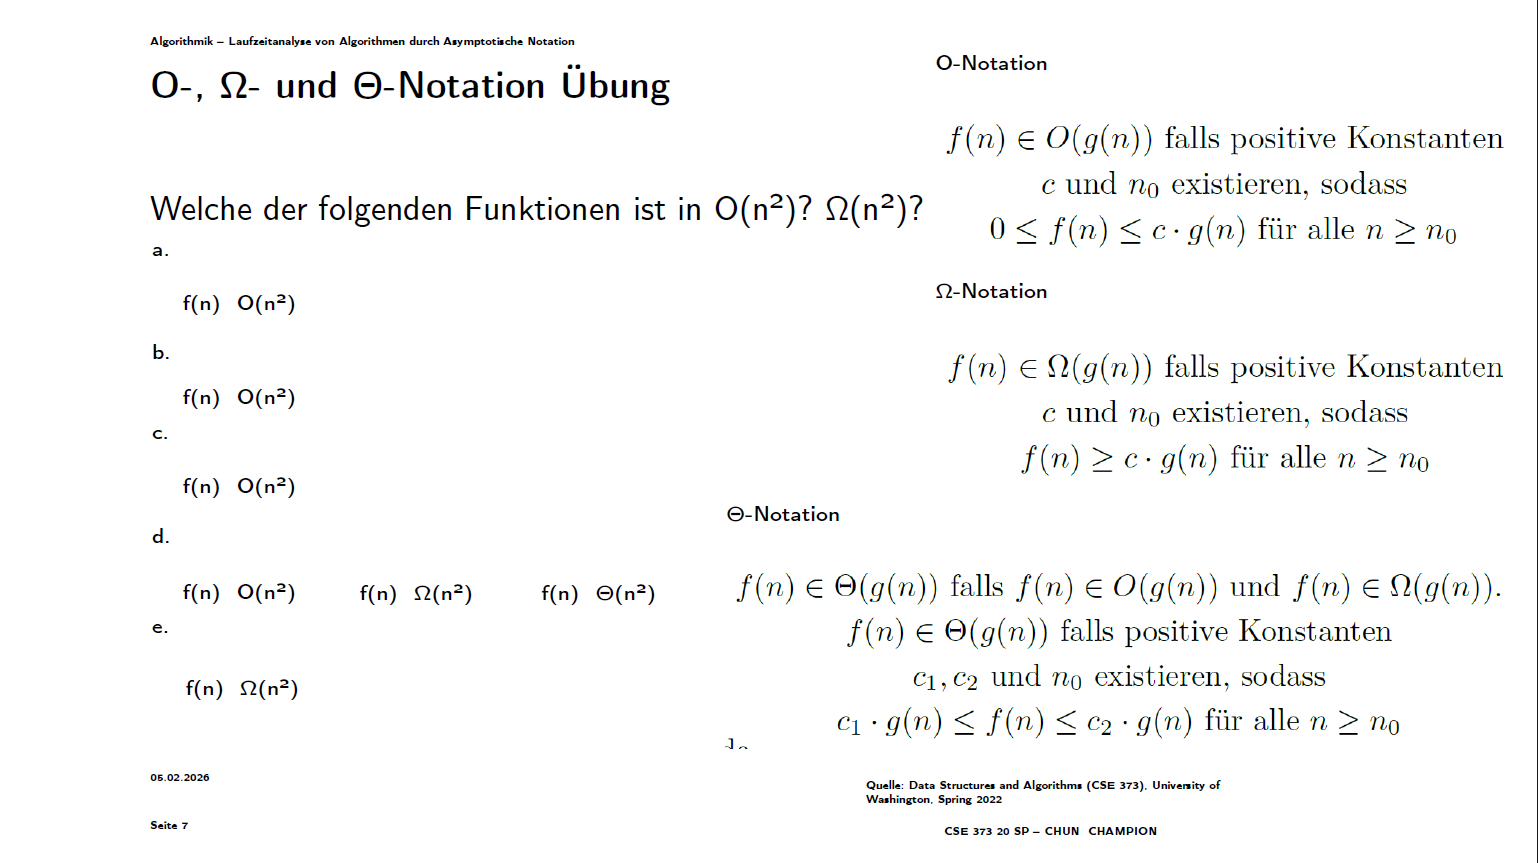
\includegraphics[width=0.95\textwidth]{img/Slide_7_non_grp_Latex.png}}
	
\end{figure}



\subsection{Vergleich mit bestehenden Lösungen}

Zur Einordnung der Ergebnisse wird das entwickelte System mit dem kommerziellen Konverter von {Aspose} verglichen [\cite{Aspose2026}]. Dabei zeigen sich grundlegende Unterschiede in der technologischen Herangehensweise sowie in der Qualität des generierten Codes.

Der Konverter von Aspose verfolgt einen vektorbasierten Export-Ansatz. Anstatt semantische Strukturen wie Listen oder Textblöcke zu erkennen, wird die Folie in hunderte Einzeloperationen zerlegt. Das Tool nutzt die {picture}-Umgebung und {\textbackslash put}-Befehle, um jedes Zeichen einzeln auf einer absoluten Koordinate zu platzieren. Grafische Elemente werden über {tikzpicture}-Scopes und {filldraw}-Befehle rekonstruiert.\\

 Ein wesentlicher Vorteil des Aspose-Konverters liegt in der hohen visuellen Genauigkeit. Da jedes Element pixelgenau positioniert wird, entspricht das Layout exakt der ursprünglichen PowerPoint-Folie. Auch komplexe Shapes, Design-Templates und Farbeinstellungen werden übernommen.

Demgegenüber stehen jedoch signifikante Nachteile in der Nutzbarkeit des Codes: 
\begin{itemize} 
	\item Da kein zusammenhängender Text, sondern Fragmente auf Koordinaten generiert werden, ist der Code für eine manuelle Nachbearbeitung unbrauchbar. Es existieren keine logischen LaTeX-Umgebungen.
	 \item Zwar werden Bilder im Code referenziert, jedoch findet oft keine Extraktion der Bilddateien statt, wodurch diese im finalen PDF fehlen.
	  \item Trotz der exakten Koordinaten kommt es häufig zu Verschiebungen bei Schriftarten und Textabständen, was das Schriftbild unruhig wirken lässt.
 \end{itemize}

Im direkten Vergleich zwischen dem Resultat des Referenz-Tools (Abbildung \ref{fig:vergleich_Aspose}) und dem hier entwickelten System (Abbildung \ref{fig:vergleich_mine_converter}) wird der konzeptionelle Gegensatz beider Ansätze deutlich. Während das Vergleichstool eine pixelgenaue, aber nicht editierbare Repräsentation erzielt, fokussiert sich das entwickelte System auf die Wiederherstellung logischer Strukturen. Obwohl der LLM-basierte Ansatz die ursprüngliche Designstruktur nicht identisch reproduziert, bleibt die semantische Informationsdichte, insbesondere bei Texten und Bildern, erhalten. Das Resultat ist ein wissenschaftlich nutzbares {LaTeX}-Dokument, das im Gegensatz zur rein visuellen Kopie eine einfache manuelle Weiterverarbeitung ermöglicht.

\begin{figure}[H]
	\centering
	
	\caption{Resultat des Aspose-Konverters}
	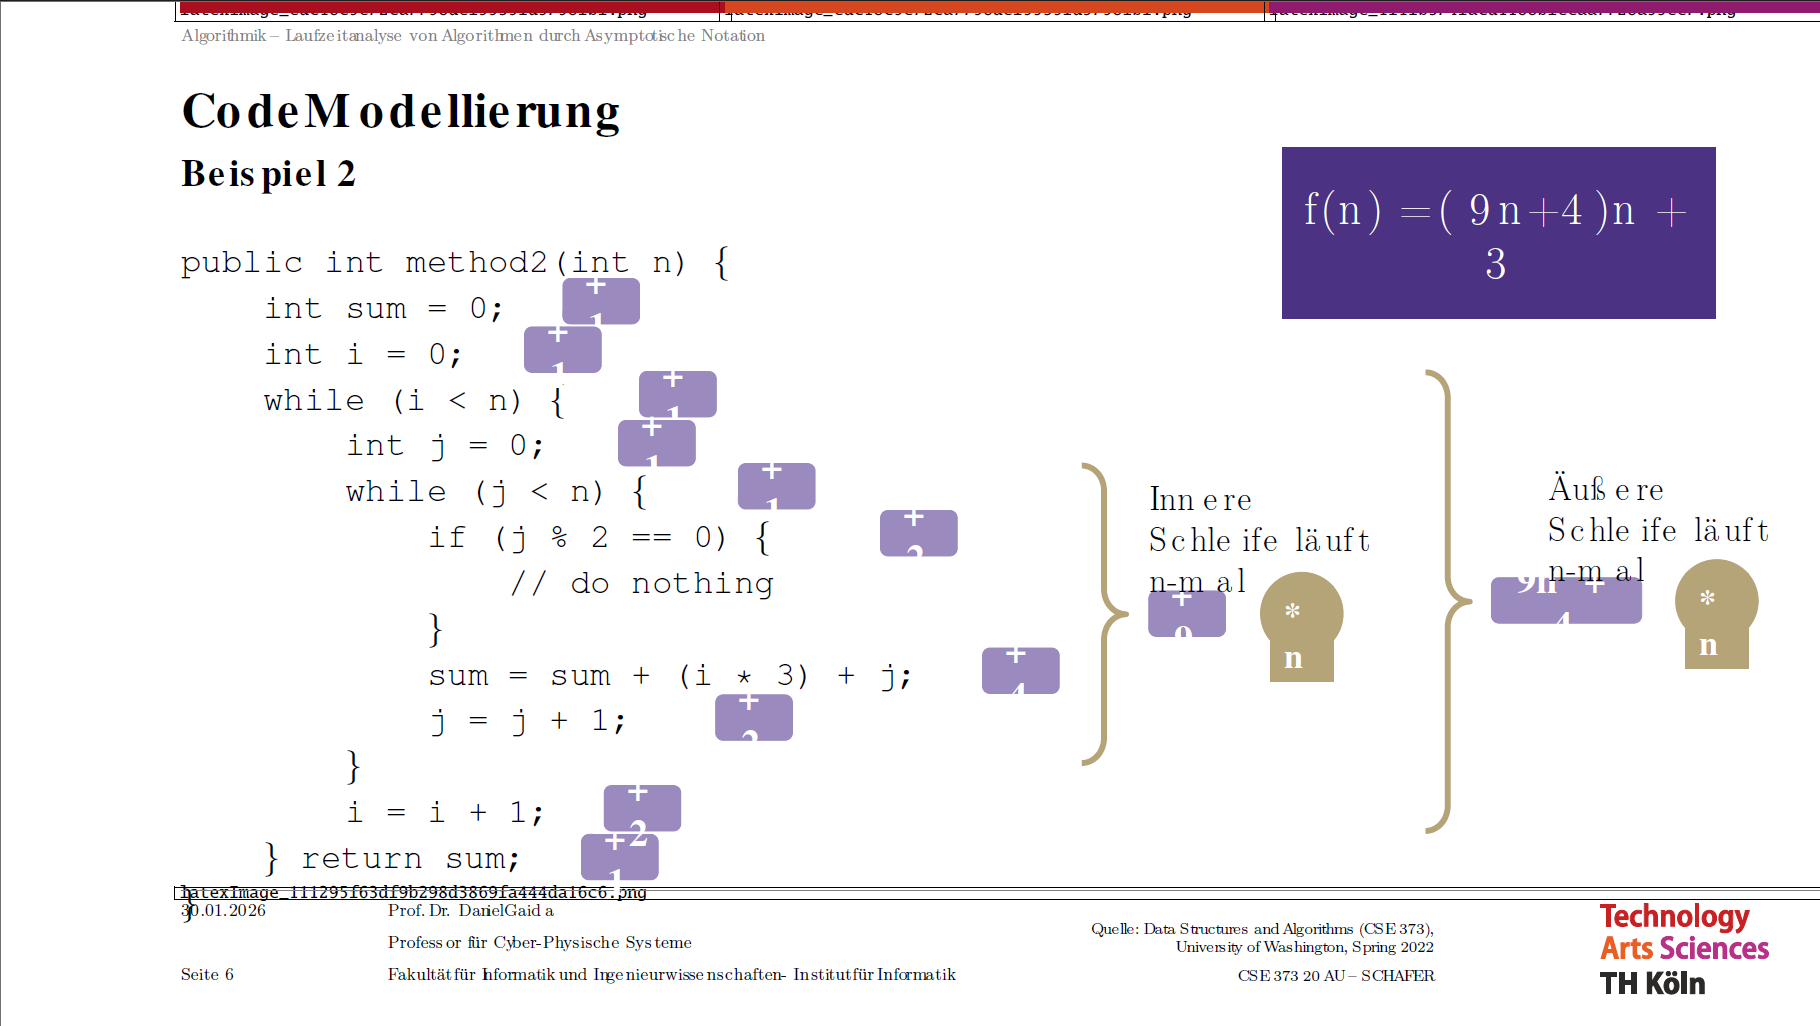
\includegraphics[width=0.9\textwidth]{img/vergleich_Aspose.png}
	\label{fig:vergleich_Aspose}
	
	\vspace{2em} 
	
	
	\caption{Resultat des eigenen Systems}
	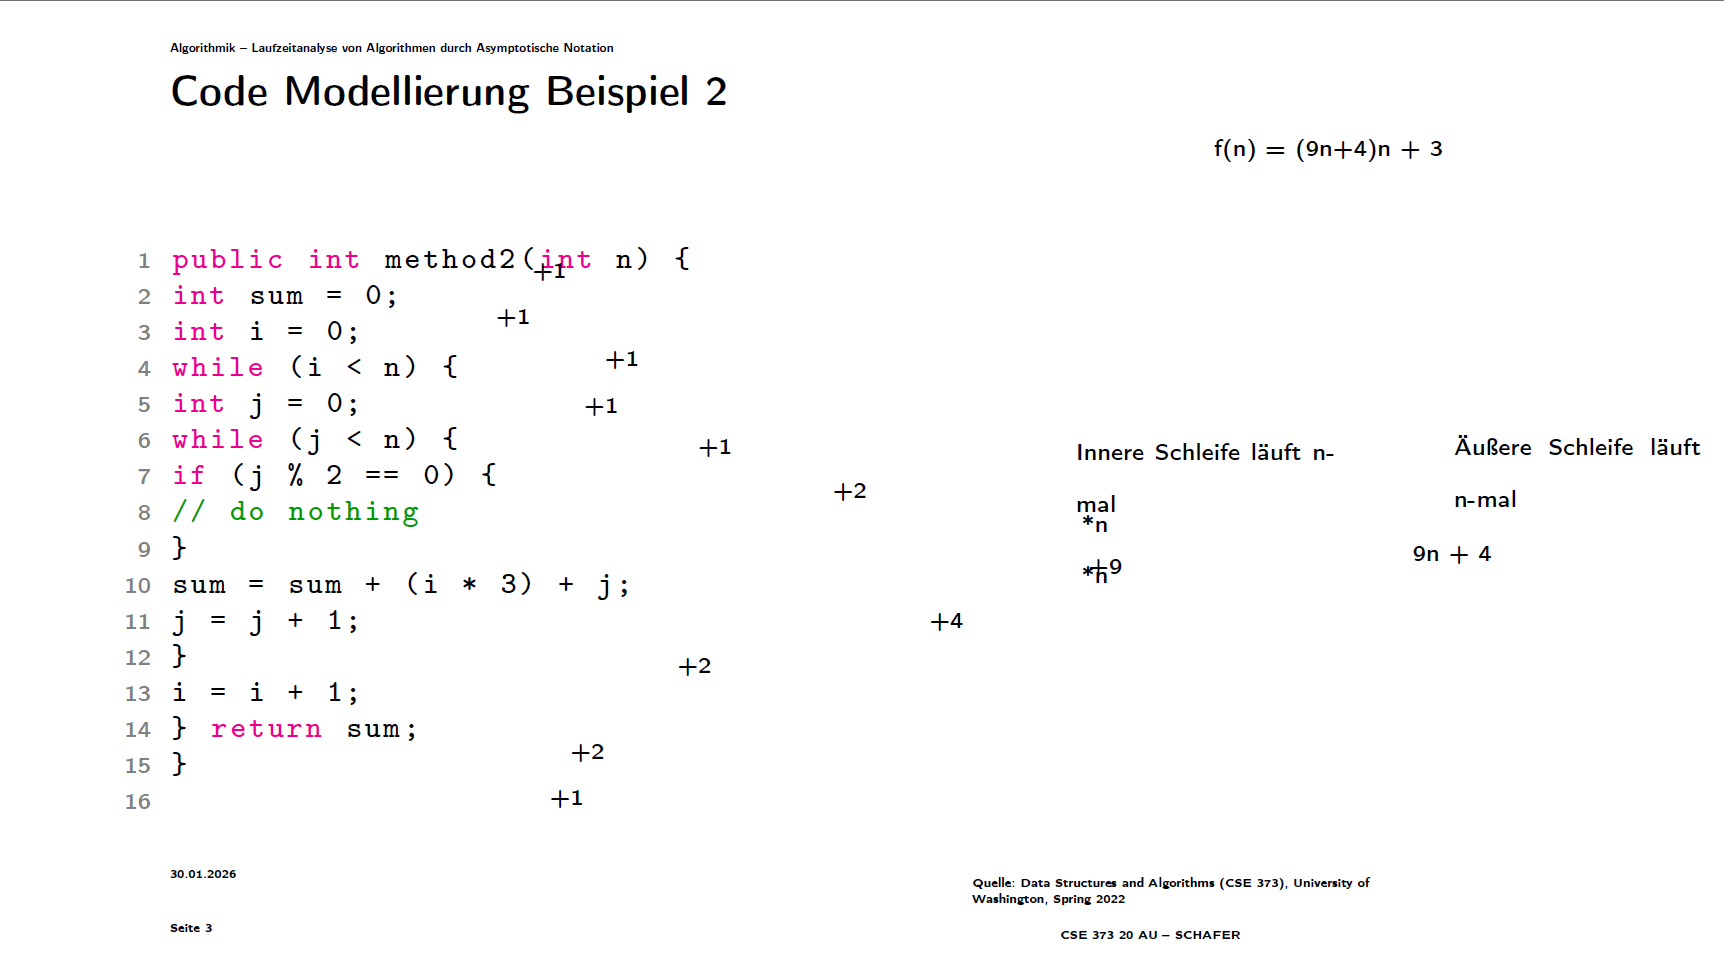
\includegraphics[width=0.9\textwidth]{img/vergleich_mine_converter.png}
	\label{fig:vergleich_mine_converter}
\end{figure}

\section{Fazit}

\subsection{Zusammenfassung der Erkenntnisse}
Ziel dieser Arbeit war die Entwicklung einer automatisierten Pipeline zur Konvertierung von PowerPoint-Präsentationen in LaTeX-Beamer-Code. Der implementierte Ansatz, der eine hybride Architektur aus klassischer Datenextraktion und generativen Sprachmodellen verfolgt, konnte die Machbarkeit dieses Vorhabens grundsätzlich bestätigen, zeigte jedoch klare Grenzen der aktuellen Technologien.


\subsubsection{Reflexion des KI-Einsatzes}
Trotz der Begeisterung für den Einsatz künstlicher Intelligenz in der Softwareentwicklung zeigt dieses Projekt, dass Large Language Models keine Universalwerkzeuge für komplexe, deterministische Probleme sind – insbesondere wenn es um die präzise Layout-Konstruktion in der UI geht.\\


Die größte Herausforderung bestand in der räumlichen Rekonstruktion. Sprachmodelle arbeiten probabilistisch – sie sagen das nächste Token basierend auf Wahrscheinlichkeiten voraus. Layout-Rendering erfordert jedoch absolute Präzision.
Es zeigte sich, dass das Modell selbst bei präzisen Prompt-Anweisungen dazu neigt, Daten zu ,,halluzinieren``. Für Aufgaben, die feste Regeln erfordern, sind klassische, imperative Algorithmen daher durchaus noch eine Überlegung wert.\\


Ein paradoxer Effekt zeigte sich bei der Nutzung des Frameworks {Docling}. Obwohl dieses Tool explizit dafür konzipiert ist, Dokumente für die KI-Verarbeitung aufzubereiten, lieferte es für diesen spezifischen Anwendungsfall ein Übermaß an Informationen. Die generierten Datenstrukturen waren derart mit redundanten Daten überfrachtet, dass sie das Kontextfenster des Modells belasteten und eine aufwendige manuelle Bereinigung des JSON-Outputs erzwangen.


\subsection{Dezentrale Ansätze}

Trotz der genannten Vorteile unterliegt die lokale Inferenz physischen Hardware-Limitierungen. Modelle mit hoher Parameteranzahl stoßen auf Standard-Systemen an Kapazitätsgrenzen, was die Verarbeitungszeit verlängert oder die Programmausführung aufgrund von Ressourcenengpässen gänzlich unterbindet. Einen Lösungsansatz bieten dezentrale Netzwerke wie \textit{gonka.ai} \citep{GonkaAI}.\\

Anstatt Rechenleistung exklusiv von einem einzelnen Unternehmen zu beziehen, werden hier verteilte Infrastrukturen erprobt. Plattformen wie gonka.ai basieren auf einem Protokoll, das ungenutzte GPU-Ressourcen einer Vielzahl unabhängiger Teilnehmer bündelt und koordiniert zur Verfügung stellt. Dies adressiert das Problem mangelnder lokaler Rechenkapazität, ohne die Souveränität über die Daten wieder vollständig an einen zentralen Großkonzern abzutreten. Solche dezentralen Architekturen könnten langfristig die Basis für unabhängige Open-Source-Tools bilden, da sie die Skalierbarkeit von Cloud-Lösungen mit dem Prinzip technologischer Autonomie verbinden.

\subsection{Anwendungspotenzial}
In der aktuellen Ausprägung wird die Pipeline primär als terminalbasierte Python-Applikation gesteuert. Während dies für die Validierung des technischen Konzepts ausreicht, stellt die fehlende grafische Benutzeroberfläche keine benutzerfreundliche Anwendung dar. Ein zentrales Ziel zukünftiger Versionen ist daher die Implementierung einer Steuerungsebene, die komplexe Konfigurationen – wie die Auswahl von Quell- und Zielverzeichnissen oder die Modellwahl – intuitiv zugänglich macht.

Ein weiterer Vorteil einer UI liegt in der gezielten Fehlerdiagnose. Anstatt systemnahe Logs auszugeben, könnten syntaktische Konflikte im LaTeX-Code visuell hervorgehoben und durch den Nutzer direkt korrigiert werden. Ergänzend dazu wäre ein User-Ansatz sinnvoll: Hierbei erhält der Nutzer die Möglichkeit, die berechneten Koordinaten der Zwischenrepräsentation vor der finalen Inferenz zu validieren. Dies würde es ermöglichen, die im Kapitel 4.1.1 identifizierten geometrischen Inkonsistenzen bei verschachtelten Gruppen manuell zu bereinigen, bevor die KI mit der Generierung des Zielcodes beginnt. Dies sichert die Layout-Treue auch in Fällen, in denen die automatisierte Extraktion an ihre strukturellen Grenzen stößt.

\subsection{Abschließende Betrachtung}
Die Arbeit zeigt, dass ein intelligenter Konverter mehr erfordert als nur ein leistungsfähiges Sprachmodell. Die Qualität des Outputs hängt maßgeblich von der Vorverarbeitung der Daten ab. Ein System, das die Stärken deterministischer Skripte mit der Flexibilität generativer KI vereint, stellt den vielversprechendsten Weg dar, um den manuellen Aufwand bei der Konvertierung komplexer Dokumente auf ein Minimum zu reduzieren.


	
	\newpage
	\pagenumbering{gobble}
	 Bei der Erstellung dieser Arbeit wurden KI-gestützte Werkzeuge zur Unterstützung bei der Strukturierung und zur sprachlichen Optimierung eingesetzt. Die inhaltliche Kontrolle und die finale Textfassung liegen vollständig beim Autor.
		\newpage
	
\bibliographystyle{natdin}
\bibliography{Literaturverzeichnis}
\addcontentsline{toc}{section}{Literaturverzeichnis}
\end{document}